\section{Quorum Systems}

In chapters before, we took decisions based on a majority-approach: if $\lfloor n/2 \rfloor + 1$ nodes decide for a value, clearly all nodes must decide for that value. This is very fault tolerant, but highly inefficient and not scalable at all! Instead, we will look at so called \textbf{quorum}. \medskip

Let $V = \{v_1, ..., v_n\}$ be a set of nodes. A quorum $Q \subseteq V$ is a subset of these nodes s.t. every two quorums intersect. When a quorum system is being used, a client selects a quorum $Q$, acquires a lock on all nodes of $Q$ and when done leases all locks again. No matter which quorum is chosen, its nodes will intersect with each other quorum. \medskip

A quorum system $S$ is called \textbf{minimal} if $\forall Q_1, Q_2 \in S : Q_1 \not\subset Q_2$. The simplest quorum system imaginable consists of just one quorum, which in turn just consists of one server. It is known as \textbf{Singleton}. In the \textbf{Majority quorum system}, every quorum has $\lfloor n/2 \rfloor + 1$ nodes.


\subsection{Load and Work}

An access strategy $Z$ defines the probability $P_Z(Q)$ of accessing a quorum $Q \in S$ s.t. $\sum_{Q \in S} P_Z(Q) = 1$. We can define two measurements for quorum systems: \medskip

\textbf{Load}:
\begin{itemize}
	\item The load of access strategy $Z$ on a node $v_i$ is 
		  $$L_z(v_i) = \sum_{Q \in S, v_i \in Q} P_Z(Q)$$
		  The load is the probability that $v_i \in Q$ if $Q$ is sampled from $S$.
		  
	\item The load induced by access strategy $Z$ on a quorum system $S$ is the maximal load induced by $Z$ on any node in $S$:
		  $$L_Z(S) = \max_{v_i \in S} L_Z(v_i) $$
	
	\item The load of a quorum system $S$ is:
	 	  $$L(S) = \min_Z L_Z(S)$$
\end{itemize}

\textbf{Work}
\begin{itemize}
	\item The work of a quorum $Q \in S$ is the number of nodes in $Q$:
		  $$W(Q) = |Q|$$
	
	\item The work induced by access strategy $Z$ on a quorum system $S$ is the expected number of nodes accessed:
		  $$W_Z(S) = \sum_{Q \in Z} P_Z(Q) \cdot W(Q)$$
		
	\item The work of a quorum system $S$ is: 
		  $$W(S) = \min_Z W_Z(S)$$
\end{itemize}

Note that you cannot choose different access strategies $Z$ for work and load, you have to pick a single $Z$ for both. If every quorum $Q$ in a quorum system $S$ has the same number of elements, $S$ is called \textbf{uniform}. \medskip

Let $S$ be a quorum system. Then $L(S) \geq 1 / \sqrt{n}$ holds.


\subsection{Grid Quorum System}

We try to achieve this lower bound for the load with so called grid quorum systems. Assume $\sqrt n \in \N$, then arrange the $n$ nodes in a $\sqrt n \times \sqrt n$ grid. The basic grid quorum consists of $\sqrt n$ quorums, each containing the full row and column $i$.
\begin{center}
	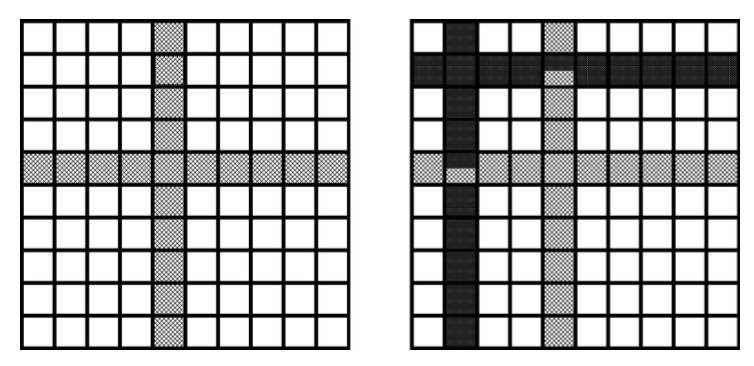
\includegraphics[width=0.6\linewidth]{grid_quorum.png}
\end{center}

However, with the simple quorum system, two quorums intersect at two nodes. They could enter a deadlock, if both quora try to get locks at the same time. By introducing some kind of ordering (e.g. the one which holds the highest lock, i.e. the one with the right-most lock in the last row, will get the lock), we can solve this problem. There are different quorum systems which only intersect in one node, e.g. the ones below:
\begin{center}
	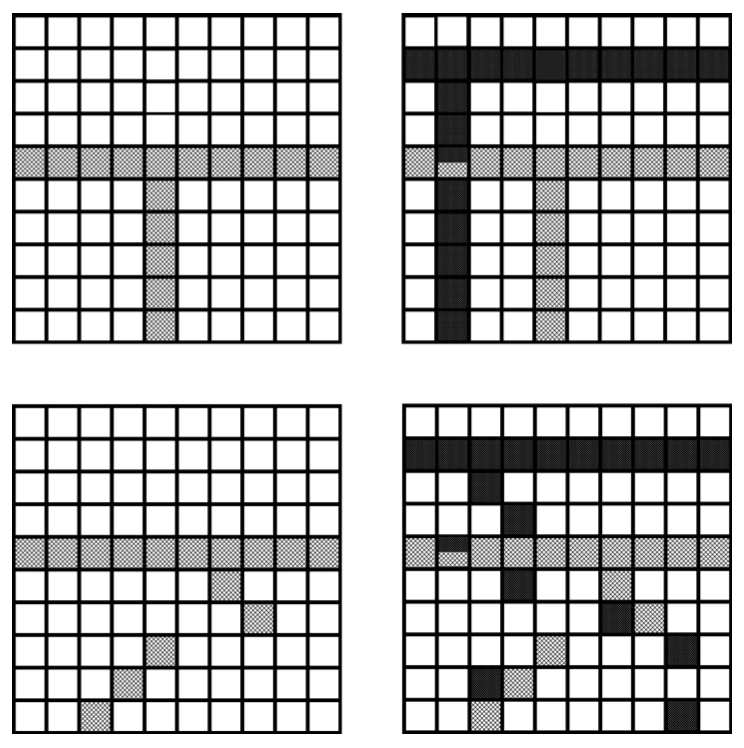
\includegraphics[width=0.6\linewidth]{grid_quorum2.png}
\end{center}

In the script, there is a detailed algorithm for locking strategies that prevent deadlocks. There are also other problems, e.g., what happens when a quorum holds locks and crashes? Instead of locks we could e.g. use leases instead of locks (which have a time out).


\subsection{Fault Tolerance}

If any $f$ nodes from a quorum system $S$ can fail s.t. there is still a quorum $Q \in S$ without failed nodes, then $S$ is $f$-resilient. The largest such $f$ is the resilience $R(S)$. \medskip

If $S$ is a Grid quorum system where each of the $n$ quorums consists of a full row and a full column, S has a re- silience of $\sqrt n - 1$: Either, all $\sqrt n$ nodes on the diagonal fail. Else, no matter which $\leq \sqrt n - 1$ nodes fail, there is always a row and column without failed nodes. \medskip

Assume that every node works with a fixed probability $p$. The failure probability $F_p(S)$ of a quorum system $S$ is the probability that at least one node of every quorum fails. The asymptotic failure probability is $F_p(S)$ for $n \to \infty$. \medskip

We have proven the following asymptotic failure probabilities:
\begin{itemize}
	\item Majority quorum system: failure probability 0
	\item Grid quorum system: failure probability 1
\end{itemize}
As we can see, we have a system with optimal load and one with fault-tolerance. If we want to achieve both, we need B-Grind quorum systems. \medskip

Consider $n = dhr$ nodes, arranged in a rectangular grid with $h \cdot r$ rows and $d$ columns. Each group of $r$ rows is a band, and $r$ elements in a column restricted to a band are called a mini-column. A quorum consists of one mini-column in every band and one element from each mini-column of one band. Thus, every quorum has $d + hr - 1$ elements. The B-Grid quorum system consists of all such quorums.
\begin{center}
	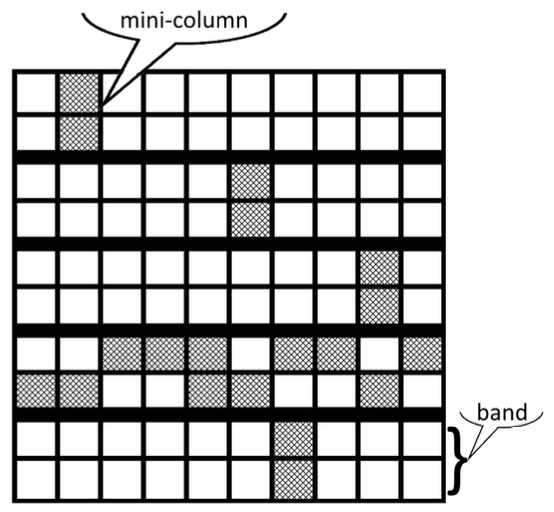
\includegraphics[width=0.42\linewidth]{b-grid-quorum.png}
\end{center}

Indeed, the asymptotic failure probability of the B-Grid quorum system is 0.
\begin{center}
	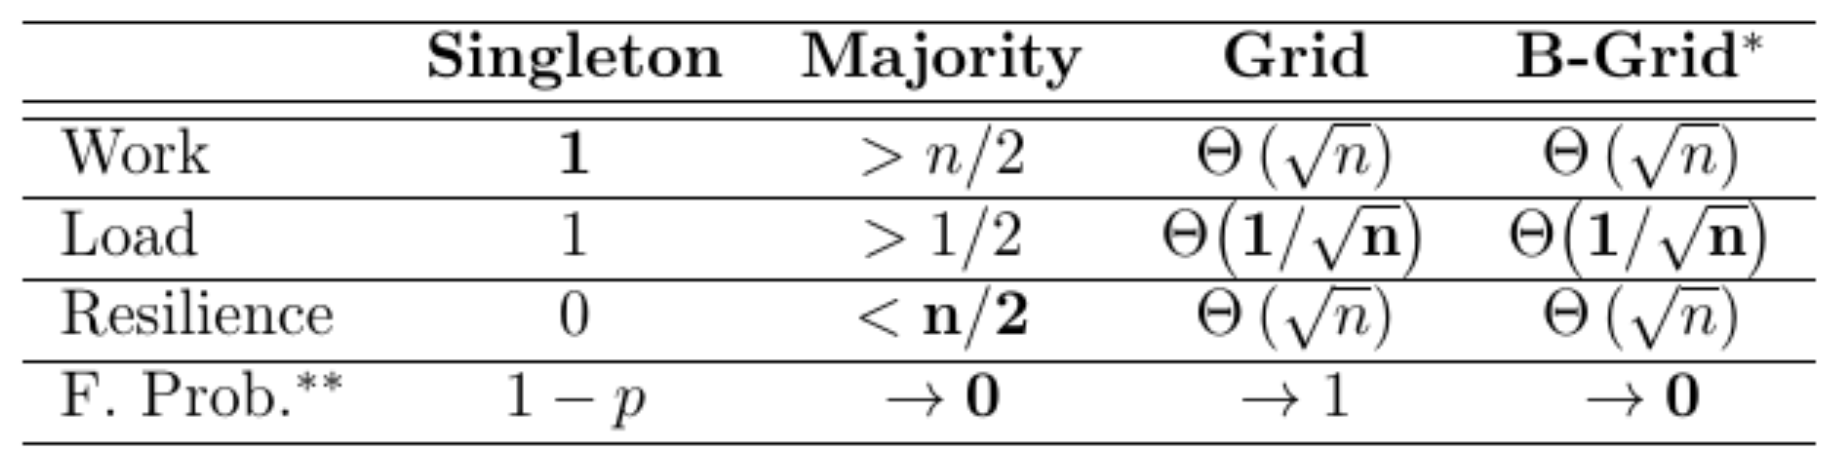
\includegraphics[width=\linewidth]{quorums.png}
\end{center}


\subsection{Byzantine Quorum System}

While failed nodes are bad, they are still easy to deal with: just access another quorum where all nodes can respond! Byzantine nodes make life more difficult. \medskip

A quorum system $S$ is $f$-disseminating if the intersection of two different quorums always contains $f + 1$ nodes (1), and for any set of $f$ byzantine nodes, there is at least one quorum without byzantine nodes (2). If we have some authentication mechanism (the data is self-verifying) in our system, then (1) is strong enough as the correct node could verify the data. If this does not hold, then we need another mechanism. \medskip

A quorum system $S$ is $f$-masking if (1) the intersection of two different quorums always contains $2f + 1$ nodes and (2) for any set of $f$ byzantine nodes, there is at least one quorum without byzantine nodes. The idea behind (1) is that $f + 1$ nodes can outvote all the byzantine nodes. Masking quorum systems need more than $4f$ nodes.\medskip

The loads for these systems are $L(S) \geq \sqrt{(f+1)/}$ for the $f$-disseminating and $L(S) \geq \sqrt{(2f+1)/2}$ for the $f$-masking. \medskip

A $f$-masking Grid quorum system is constructed as the grid quorum system, but each quorum contains one full column and $f + 1$ rows of nodes, with $2f + 1 \leq \sqrt{n}$. In such a system, two quorums overlap by their columns intersecting each others rows – the overlap is thus at least $2f + 2$ nodes. The $f$-masking Grid nearly hits the lower bound, but is not optimal.
\begin{center}
	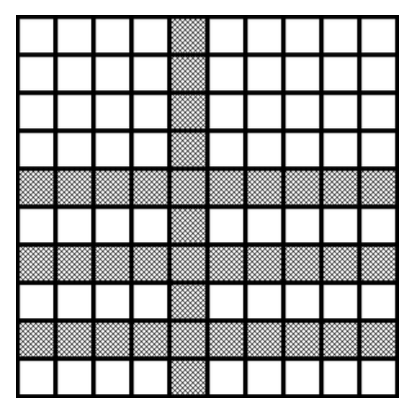
\includegraphics[width=0.42\linewidth]{f_quorum.png}
\end{center}

The $M$-Grid quorum system on the other hand hits the lower bound: it is constructed as the grid quorum system, but each quorum contains $\sqrt{f + 1}$ rows and $\sqrt{f + 1}$ columns of nodes, with $f \leq \frac{\sqrt{n-1}}{2}$. For both of these systems, the load is in $\Theta(\sqrt{f/n})$.
\begin{center}
	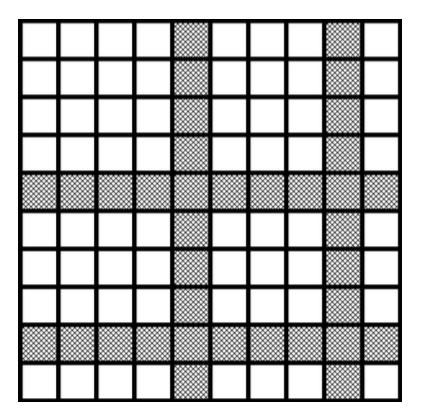
\includegraphics[width=0.42\linewidth]{M-quorum.png}
\end{center}

We achieved nearly the same load as without byzantine nodes! However, as mentioned earlier, what happens if we access a quorum that is not up-to-date, except for the intersection with an up-to-date quorum? \medskip

We might want to ensure that the number of correct up-to-date nodes accessed will be larger than the number of out-of-date nodes and byzantine nodes. \medskip

A quorum system $S$ is $f$-opaque if the following two properties hold for any set of $f$ byzantine nodes $F$ and any two different quorums $Q_1, Q_2$:
$$|(Q_1 \cap Q_2) / F| > |(Q_2 \cap F) \cup (Q_2 / Q_1)| $$
$$(F \cap Q) = \emptyset \text{ for some } Q \in S$$

For a $f$-opaque system, we need $n > 5f$. For a $f$-opaque quorum system $S$, we also have $L(S) \geq 1/2$.



